\section{Grapped Phases II}
\subsection{Review of Last Lecture}
Last time, we discussed:
\begin{enumerate}
    \item Two local gapped Hamiltonians as belonging to the same phase if they can be connected by a local (short-ranged, or superpolynomial decaying interactions), gapped path $\set{H(s): 0 \leq s \leq 1}$.
    \begin{center}
        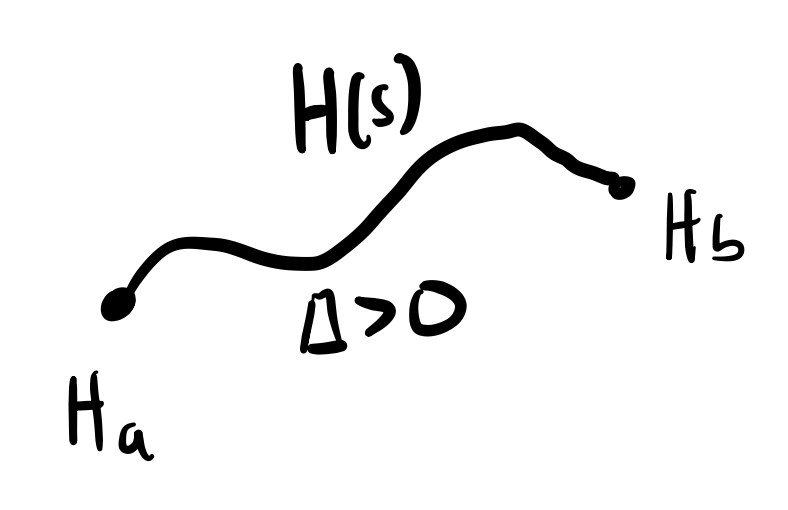
\includegraphics[scale=0.35]{Lectures/Images/lec11-interpolation.png}
    \end{center}
    \item A local unitary transformation is a unitary of the form:
    \begin{equation}
        U(T) = \mathcal{T}\exp(-i\int_0^T H(t)dt)
    \end{equation}
    \item Lieb-Robinson bound; local unitaries only spread operators by a distance of order $v_{LR}T$ where $v_{LR}$ is the Lieb-Robinson velocity. The sketch we had was that of $O$ supported in $R$, $U^\dag O U$ supported in a radius $v_{LR}T$ beyond $R$ (up to superpolynomially decaying tails).
    \begin{center}
        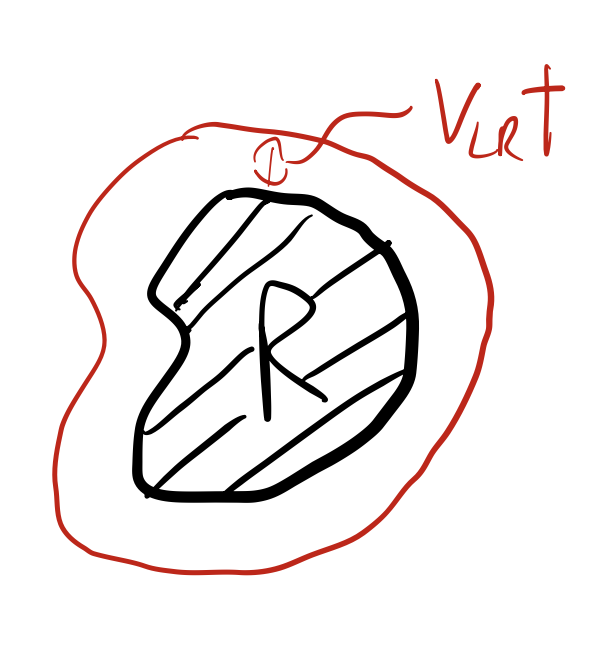
\includegraphics[scale=0.35]{Lectures/Images/lec11-LRbound.png}
    \end{center}
    A note: in the important special case of a quantum circuit\footnote{Though, in many parts of the literature people treat a quantum circuit and a finite depth local unitary as synonymous.}, we find that the operator $O$ is \emph{strictly} supported in a lightcone (no tails):
    \begin{center}
        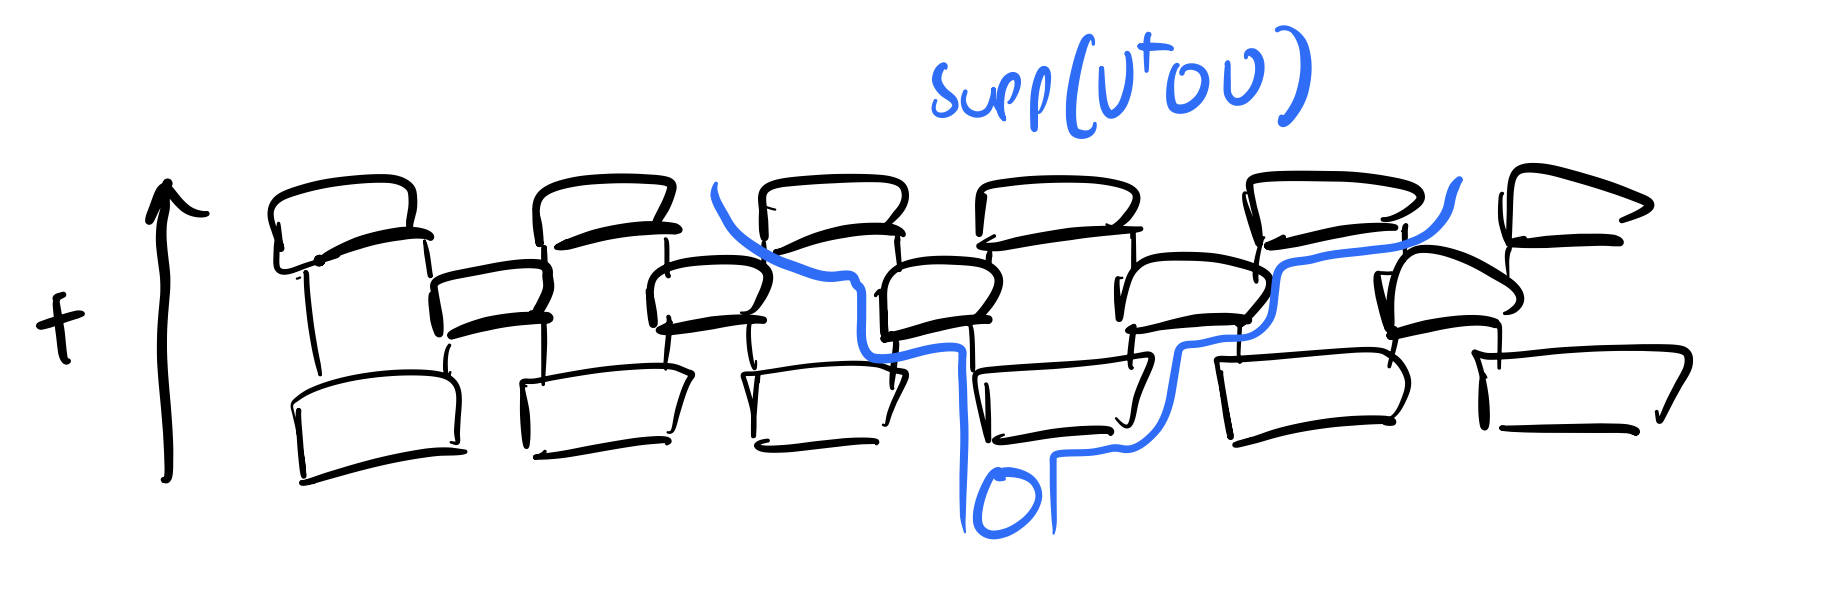
\includegraphics[scale=0.35]{Lectures/Images/lec12-lightcone.png}
    \end{center}
\end{enumerate}

\subsection{Quasi-Adiabatic Continuation}
The reference is Hastings, \texttt{arXiv/1008.5137}. We can think of this as a confinement of adiabatic evolution - we use this as in adiabatic evolution we can have badly behaved error terms, have to wait a very long time etc. In this sense quasi-adiabatic continuation has nicer properties. Here, we discuss exact quasi-adiabatic continuation, where there is no error whatsoever.

\textit{Theorem (Hastings).} For any smooth family of of local gapped Hamiltonians\footnote{Note that this result holds equally as well in the thermodynamic limit and for finite system size.} $\set{H(s): 0 \leq s \leq 1}$ with unique ground states $\ket{\Omega(s)}$, there exists a local unitary transformation $U$ such that $U\ket{\Omega(0)} = \ket{\Omega(1)}$\footnote{If you allow for superpolynomial tails, this is exact. For exponential tails, you may get errors.}

Some remarks:
\begin{enumerate}
    \item $U$ is \emph{not} generated by $H(s)$. Instead it is generated by another Hermitian operators $D(s)$ which is defined in terms of $H(s), \p_sH(s)$, which is called the generator of QAC.
    \item More generally, if $H(s)$ has multiple ground states $\set{\ket{\Omega_i(s)}}$ then, the same construction applies, with:
    \begin{equation}
        UP(0)U^\dag = P(1)
    \end{equation}
    with $P(s)$ the ground-state projector $P(s) = \sum_i \dyad{\Omega_i(s)}{\Omega_i(s)}$.
    \begin{center}
        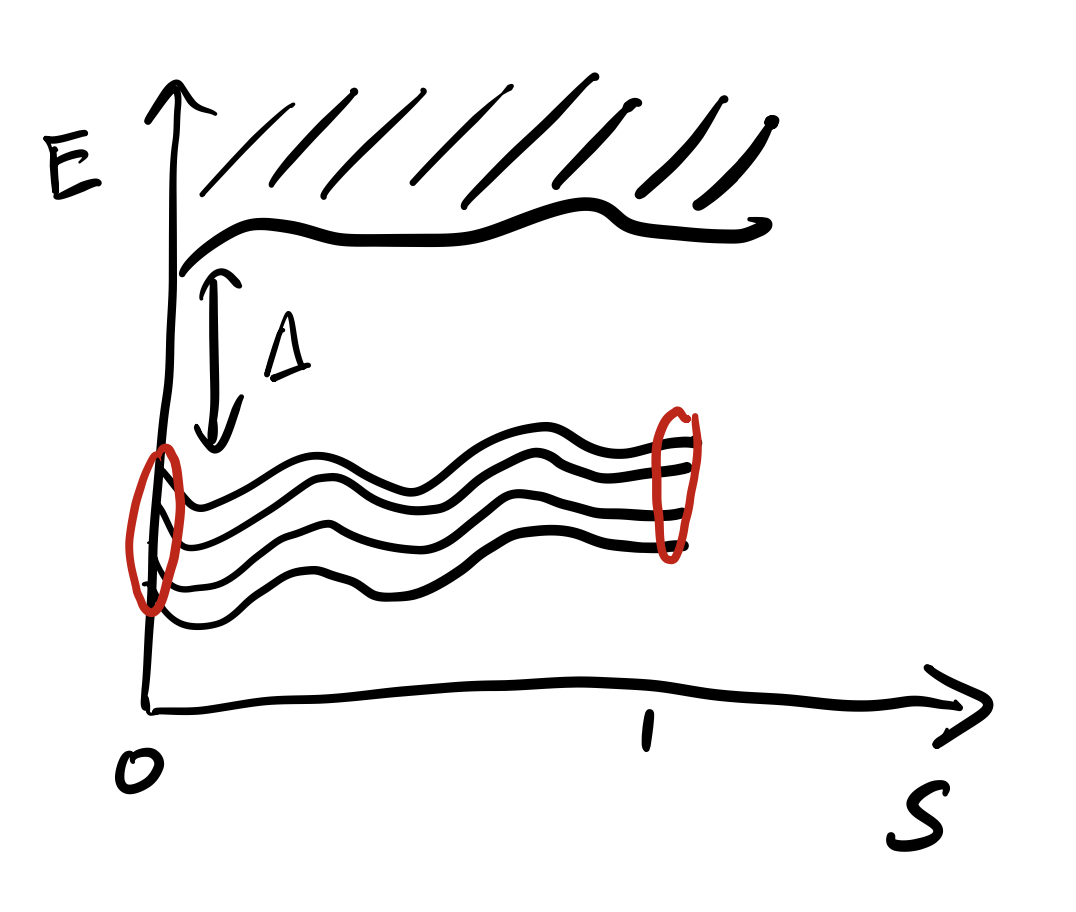
\includegraphics[scale=0.35]{Lectures/Images/lec12-preservinggroundspace.png}
    \end{center}
\end{enumerate}

\subsection{Application 1 - Another definition of gapped phases}
What does QAC teach us about gapped phases? One application is that it allows us to define gapped phases in another way. We see this as follows:

\begin{enumerate}
    \item If two Hamiltonians $H_a, H_b$ belong to the same gapped phase and have unique ground states $\ket{\Omega_a}, \ket{\Omega_b}$, then:
    \begin{equation}
        \ket{\Omega_b} = U\ket{\Omega_a}
    \end{equation}
    for some local unitary $U$ (this comes from QAC).
    \item In fact, the converse is also true; if $\ket{\Omega_b} = U\ket{\Omega_a}$ and $\ket{\Omega_a}, \ket{\Omega_b}$ are unique gapped ground states of $H_a, H_b$ belong to the same phase.

    To show this, we need to construct an interpolation:
    \begin{equation}
        H(s) = U(s)H_aU(s)^\dag
    \end{equation}
    where:
    \begin{equation}
        U(s) = \mathcal{T}\exp(-i\int_0^{sT} \bar{H}(t)dt)
    \end{equation}
    with $\bar{H}(t)$ defined via $U$:
    \begin{equation}
        U = \mathcal{T}\exp(-i\int_0^{T} \bar{H}(t)dt)
    \end{equation}
    Then:
    \begin{enumerate}[(a)]
        \item $H(s)$ is local (Lieb-Robinson)
        \item $H(s)$ is gapped (since $H_a$ is gapped)
        \item $H(s = 0) = H_a$, and $H(s = 1) = U(s=1)H_aU(s=1)^\dag$ has $\ket{\Omega_b}$ as the ground state (not necessarily $H_b$, but has the same ground state):
        \begin{equation}
            (U(s=1)H_aU^\dag(s=1))\ket{\Omega_b} = (UH_aU^\dag)\ket{\Omega_b} = UH\ket{\Omega_a} = UE_a\ket{\Omega_a} = E_aU\ket{\Omega_a} = E_a\ket{\Omega_b}
        \end{equation}
        Then since $UH_aU^\dag$ has the same ground state as $H_b$, we can construct a gapped path $H'(s)$ connecting the two. You will verify this fact on the homework - in fact the path is just a linear interpolation:
        \begin{equation}
            H'(s) = (1-s)U H_a U^\dag + s H_b.
        \end{equation}
        The picture looks like:
        \begin{center}
            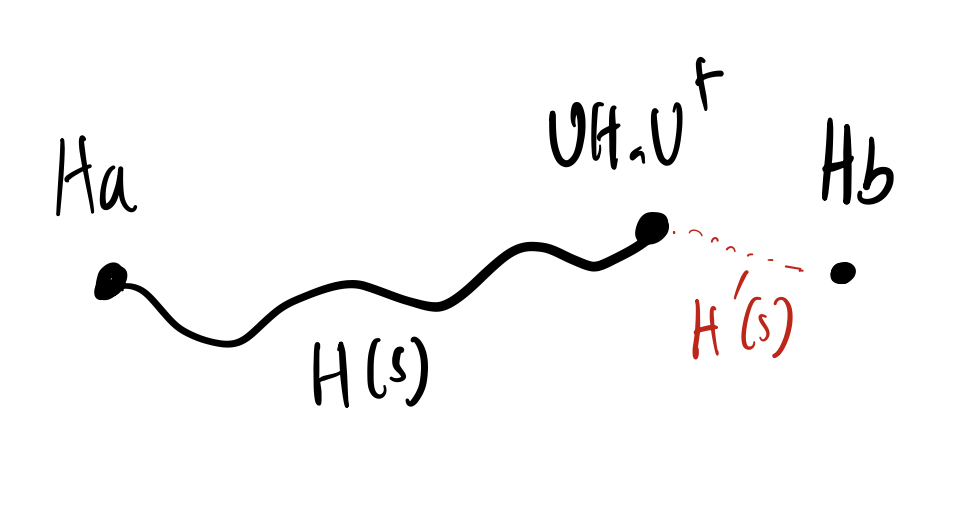
\includegraphics[scale=0.35]{Lectures/Images/lec12-connectingH.png}
        \end{center}
    \end{enumerate}
\end{enumerate}

So, to summarize, $H_a, H_b$ belong to the same phase iff $\ket{\Omega_a}, \ket{\Omega_b}$ are connected by a local unitary transformation. This tells us that gapped phases can be understood purely in terms of ground states; loosely:
\begin{equation}
    \text{gapped phases} = \frac{\set{\text{gapped ground states}}}{\text{local unitary transformations}}
\end{equation}
This is nice because the question of gapped phases reduces to the study of states modulo a local unitary transformation. In this picture, the Hamiltonian is is only useful insofar as it restricts the scope to those with a gap - for example we have critical states, which have algebraic correlations, which cannot be written as ground states of a gapped local Hamiltonian. But really from this point of view the only useful part of the Hamiltonian is that it exists, in some sense it restricts us to ``physical'' states. Some people are thinking about whether we could get rid of Hamiltonians completely, but this is an open research question.

\subsection{Application 2 - Universality within gapped phases}
Let $H$ be the toric code Hamiltonian with $\ket{\Omega}$ the ground state (let's use the infinite plane for now, so $\ket{\Omega}$ is unique). Let $W_e(\gamma), W_m(\gamma)$ be the flexible string operators that create $e, m$ excitations. Now, let's imagine that we have $\tilde{H}, \ket{\tilde{\Omega}}$ in the same phase as the toric code. Then:
\begin{equation}
    \ket{\tilde{\Omega}} = U\ket{\Omega}
\end{equation}
for some local unitary $U$.

Then, we define:
\begin{equation}
    \tilde{W}_{e/m}(\gamma) = U W_{e/m}(\gamma)U^\dag
\end{equation}
as the flexible string operators for the new state.

\begin{itemize}
    \item Let's see that these are indeed string operators; since $U$ is local, by Lieb-Robinson if $W_{e/m}(\gamma)$ is supported near a path $\gamma$ then $\tilde{W}_{e/m}(\gamma)$ is still supported near that path, just spread out a little (bounded by the LR velocity).

    \begin{center}
        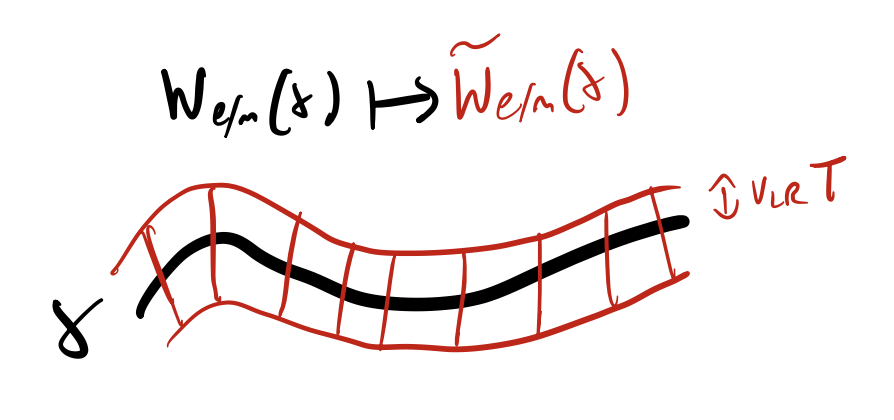
\includegraphics[scale=0.35]{Lectures/Images/lec12-broadstringops.png}
    \end{center}

    \item These operators are also flexible, which is easily seen by the fact that their action on $\ket{\tilde{\Omega}}$ reduces to the action on $\ket{\Omega}$:
    \begin{equation}
        \tilde{W}_{e/m}\ket{\tilde{\Omega}} = UW_{e/m}U^\dag U\ket{\Omega} = UW_{e/m}\ket{\Omega}
    \end{equation}
    \item $\tilde{W}_{e}, \tilde{W}_{m}$ obey the same algebra as $W_e, W_m$ (all of the $U$s cancel out when taking commutators).
\end{itemize}

Thus, $\tilde{W}_e, \tilde{W}_m$ create anyon excitations with the same mutual and exchange statistics as $e, m$.

This type of argument shows that anyon properties are constant throughout each gapped phase. For example, let's take the toric code model and add single site terms:
\begin{equation}
    H = -\sum_s A_s - \sum_p B_p - h_X\sum_j X_j - h_Z \sum_j Z_j
\end{equation}
now, $h_x, h_z$ are like two parameters we can vary. We then get a phase diagram consisting of two phases:

\begin{center}
    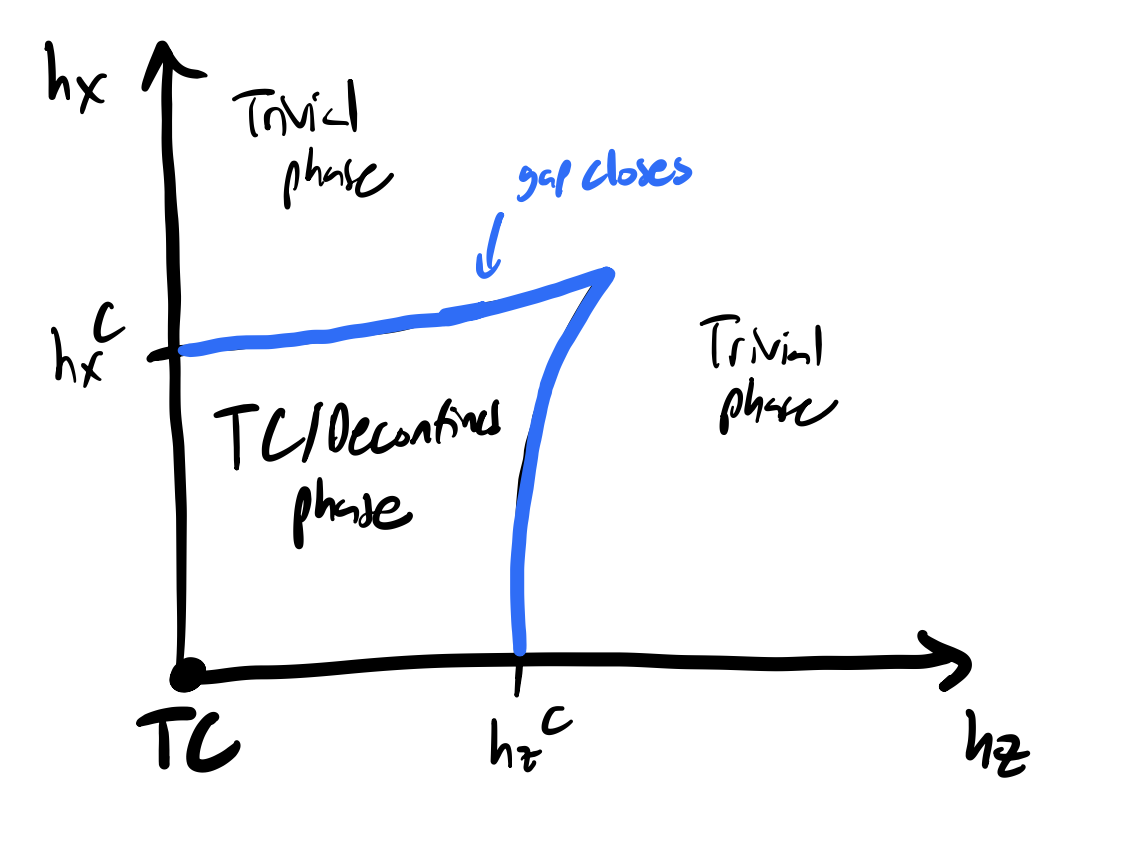
\includegraphics[scale=0.35]{Lectures/Images/lec12-TCphasediagram.png}
\end{center}

Consisting of the TC (deconfined) phase and the trivial (confined\footnote{The terminology comes from gauge theory, where this phase diagram was first deduced. }) phase. We have the gap closing along the sketched lines (where $h_x^C = h_z^C = \mathcal{O}(1)$). The trivial phase is the phase of states connected to the product state (you can see that taking $h_X \to \infty$ we just get a product state, same as $h_Z \to \infty$). We can also see that the TC and trivial phases are distinct in the sense that the former phase hosts anyons, the latter does not.

\subsection{Short-range entangled states}
\textit{Definition.} A state $\ket{\psi}$ is short-range entangled (SRE) if it can be written as:
\begin{equation}
    \ket{\psi} = U\ket{\psi_0}
\end{equation}
where $U$ is a local unitary and $\ket{\psi_0}$ is a product state.

In the context of our above phase diagram, states in the trivial phase are SRE, while states in the toric code are not (they cannot be connected to the product state via a local unitary).

Any state that is not SRE we call \emph{long-range entangled}.